\begin{mainquestion}{cstransfer}{Common Source Amplifier Transfer Characteristic}

Consider a common source (CS) amplifier as shown below. The key parameters are $V_{DD} = 10\ \text{V}$, $R_{D} = 8.5\ \text{k}\Omega$, $k_{n} = k_{n}^{\prime}\frac{W}{L} = 5\ \frac{\text{mA}}{V^{2}}$, and $V_{t} = 1\ \text{V}$. Assume $\lambda = 0$ for parts (a)-(d).

\begin{center}
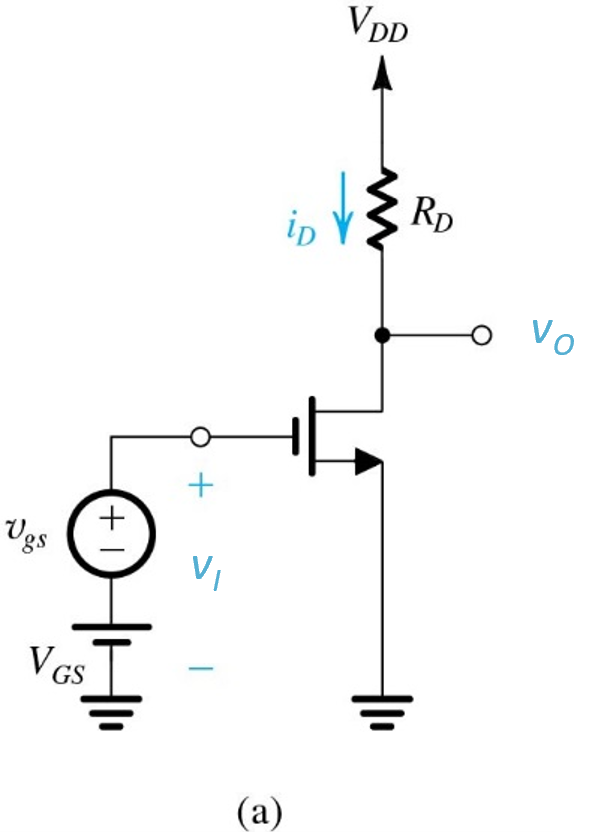
\includegraphics[width=2in]{questionbank/amplifiers/cs_transfer_characteristic/v0/Picture1.png}
\quad
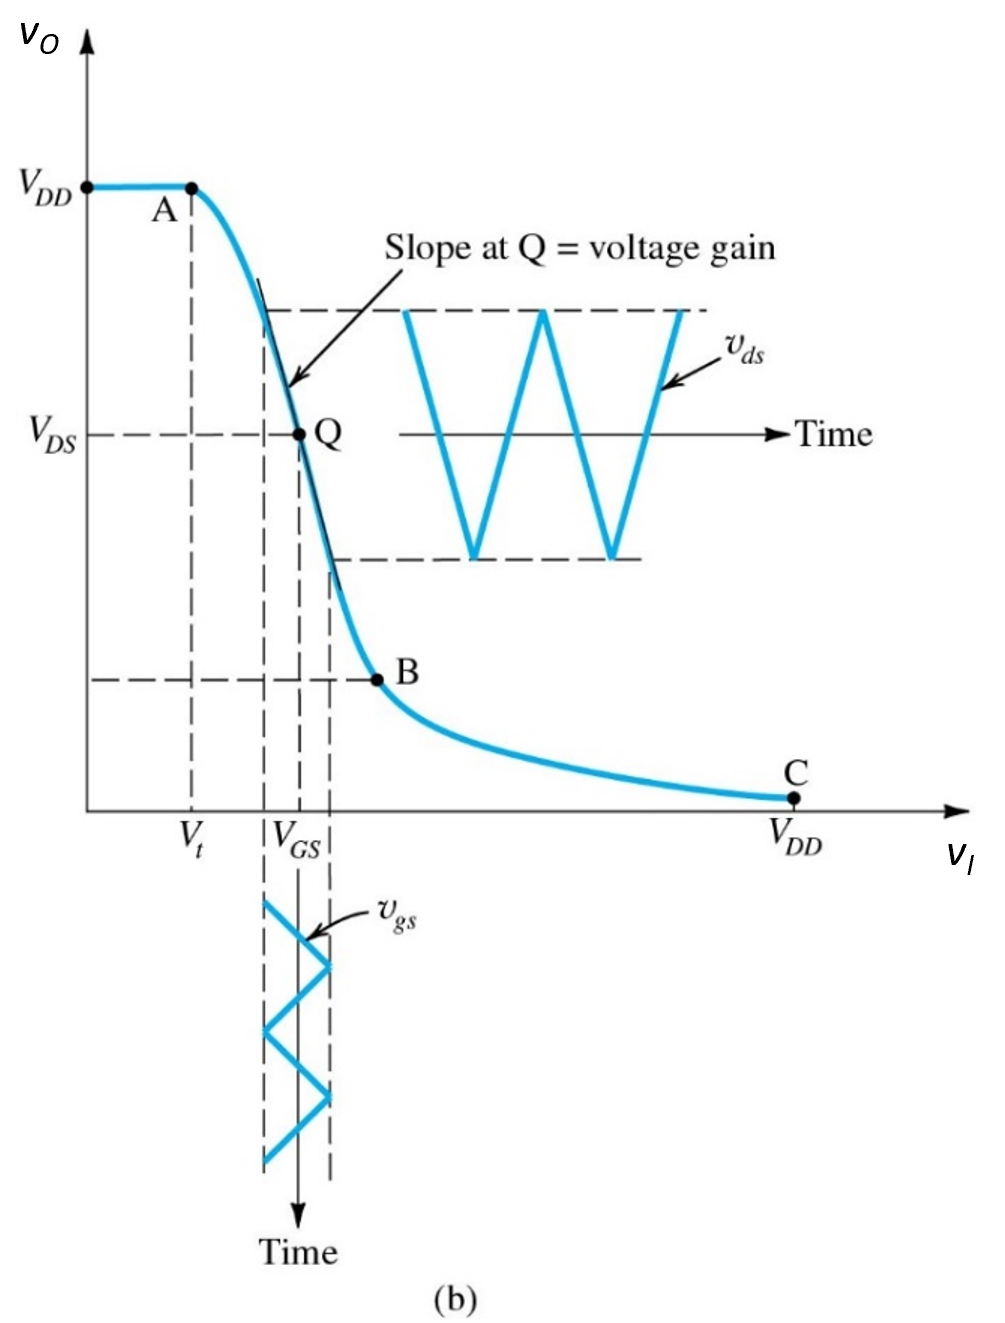
\includegraphics[width=3in]{questionbank/amplifiers/cs_transfer_characteristic/v0/Picture2.png}
\end{center}

\begin{partquestion}{findpointsab}{Find the coordinates of points A and B (i.e., $V_{I}$ and $V_{O}$) on the sketch above.}
\begin{answer}
Point A on the sketch corresponds to the moment when the transistor transitions from cut-off to saturation. This occurs when $v_{I} = v_{GS} = V_{t} = 1\ \text{V}$. At this point, current is just beginning to flow so $v_{DS} = v_{O} = V_{DD}$. So, point A is (1 V, 10 V).

Point B corresponds to the moment where the transistor goes from saturation to triode. In this case, $V_{DS} = V_{GS} - V_{t}$ so $v_{O} = v_{I} - V_{t} = v_{I} - 1\ \text{V}$. Because at point B we are at the boundary of two regions, either formula for $I_{D}$ should work (also because $\lambda = 0$, which ensures continuity between regions with our standard formulas for $I_{D}$). Choosing that of saturation gives:

\[
I_{D} = \frac{V_{DD} - v_{O}}{R_{D}} = \frac{1}{2} k \left(V_{GS} - V_{t}\right)^{2}
\]

so

\[
\frac{10 - v_{o}}{8.5} = \frac{1}{2}(5)(v_{I} - 1)^{2} = \frac{1}{2}(5)v_{O}^{2}
\]

this leads to the quadratic:

\[
2.5 v_{O}^{2} + 0.1176 v_{O} - 1.1765 = 0
\]

which has solutions $v_{O} = -0.710$ and $v_{O} = 0.663$. Only the second is a valid solution. From here, $v_{I} = v_{O} + 1 = 1.663\ \text{V}$, so point B is (1.663 V, 0.663 V).
\end{answer}
\end{partquestion}

\begin{partquestion}{biaspoint}{If the amplifier is biased to operate with an overdrive voltage $V_{OV} = V_{GS} - V_{t} = 0.4\ \text{V}$, find the bias point Q on the transfer characteristic. What is the value of $I_{D}$ when operating at the bias point Q?}
\begin{answer}
We know with this overdrive voltage level:

\[
v_{I} = V_{GS} = V_{OV} + V_{t} = 0.4 + 1.0 = 1.4\ \text{V}.
\]

We can use the same equation as in part (a) to find the output voltage:

\begin{gather*}
    \frac{10 - v_o}{8.5} = \frac{1}{2}(5)(v_I - 1)^2 = \frac{1}{2}(5)v_{OV}^2 = \frac{5}{2}(0.4)^2 = 0.4 \\
    v_o = 10 - (0.4)(8.5) = \qty{6.6}{\volt}
\end{gather*}

The point Q is therefore (1.4 V, 6.6 V). It follows that:

\[
I_{D} = \frac{10 - v_{o}}{8.5} = \frac{10 - 6.6}{8.5} = 0.4\ \text{mA}.
\]
\end{answer}
\end{partquestion}

\begin{partquestion}{maxamplitude}{At the bias point Q, what is the largest amplitude of a sine-wave voltage signal that can be applied at the input while the transistor remains in saturation? What is the peak-to-peak voltage of the output signal that results?}
\begin{answer}
Since our quiescent point Q has an input voltage which is closer to point B's input voltage than it is to point A's input voltage, a sine wave centered on point Q (about 1.4 V) will hit a limiting point at B (1.663 V) when the amplitude of that wave is $1.663 - 1.4 = 0.263\ \text{V}$. While there will be distortion due to the square-law relationship of the current in the saturation regime, it will remain in saturation. With an input sine wave of amplitude of 0.263 V, at the maximum input, the output will dip to 0.663 V (since we are touching point B). At the minimum input, the output will rise to a value determined by an input $v_{I} = 1.4 - 0.263 = 1.137\ \text{V}$ as follows:

\begin{align*}
    \frac{10 - v_o}{8.5} &= \frac{1}{2}(5)(v_I - 1)^2 \\
    10 - v_o &= \frac{1}{2}(5)(8.5)(1.137 - 1)^2 \\
    v_o &= 10 - \frac{1}{2}(5)(8.5)(0.137 - 1)^2 \\
    &= \qty{9.60}{\volt}
\end{align*}

The peak-to-peak voltage of the output signal is then $9.60 - 0.663 = 8.938\ \text{V}$.
\end{answer}
\end{partquestion}

\begin{partquestion}{gainandtransconductance}{What are the transconductance $g_{m}$ and gain $A_{v}$ at point Q? Provide the gain both in linear (V/V) and log (dB) units.}
\begin{answer}
The transconductance is:

\begin{align*}
    g_m &= k(V_{GS} - V_t) \\
    &= 5(1.4 - 1) \\
    &= \qty{2.0}{\milli\siemens}
\end{align*}

The gain (ignoring output resistance) is:

\[
A_{vo} = -g_{m} R_{D} = -2(8.5) = -17\ \frac{\text{V}}{\text{V}}
\]

which, in decibels is:

\[
A_{vo,dB} = 20\log|A_{vo}| = 20\log|17| = 24.6\ \text{dB}.
\]
\end{answer}
\end{partquestion}

\begin{partquestion}{lambdaeffect}{Now consider the MOSFET has a non-zero channel-length modulation parameter $\lambda$. What is the maximum $\lambda$ allowed so the voltage gain does not fall below 24 dB? What is the minimum output resistance $r_{o}$? (You may assume the bias point Q is not affected by $\lambda$.)  }
\begin{answer}
With output resistance, the formula for the gain is modified slightly:

\[
A_{vo} = -g_{m} \left(R_{D} \parallel r_{o}\right) = -\frac{g_{m} R_{D} r_{o}}{R_{D} + r_{o}}
\]

Because the minimum gain must be 24 dB, we have:

\begin{align*}
    20\log|A_v| &\geq 24 \\
    20\log\left(\frac{g_m R_D r_o}{R_D + r_o}\right) &\geq 24 \\
    \left(\frac{g_m R_D r_o}{R_D + r_o}\right) &\geq 10^\frac{6}{5} \\
    g_m R_D r_o &\geq 10^\frac{6}{5}R_D + 10^\frac{6}{5}r_o \\
    r_o &\geq \frac{10^\frac{6}{5}R_D}{g_m R_D - 10^\frac{6}{5}} \\
\end{align*}

Since $r_{o} = \frac{1}{\lambda I_{D}}$, we have:

\begin{align*}
    \lambda &= \frac{1}{r_o I_D} \\
    &\leq \frac{g_m R_D - 10^\frac{6}{5}}{10^\frac{6}{5}R_D I_D} \\
    &\leq \frac{(2) (8.5) - 10^\frac{6}{5}}{10^\frac{6}{5}(8.5)(0.4)} \\
    &\leq \qty{0.0214}{\per\volt} \\
\end{align*}

so, it follows that

\[
r_{o} \geq \frac{1}{\lambda_{\max} I_{D}} = \frac{1}{(0.0214)(0.4)} = 117\ \text{k}\Omega.
\]
\end{answer}
\end{partquestion}

\end{mainquestion}
